\documentclass[onecolumn, draftclsnofoot,10pt, compsoc]{IEEEtran}
\usepackage{graphicx}
\usepackage{url}
\usepackage{setspace}
\usepackage{cite}
\usepackage{geometry}
\usepackage{enumitem}
\usepackage{graphics}

\geometry{textheight=9.5in, textwidth=7in}

% 1. Fill in these details
\def \CapstoneTeamName{Audio Extravaganza}
\def \CapstoneTeamNumber{26}
\def \GroupMemberOne{Martin Barker}
\def \GroupMemberTwo{Devon Cash}
\def \GroupMemberThree{Alexander Niebur}
\def \GroupMemberFour{Mason Sidebottom}
\def \GroupMemberFive{Ben Windheim}
\def \CapstoneProjectName{Audio Extravaganza}
\def \CapstoneSponsorCompany{Oregon State University}
\def \CapstoneSponsorPerson{Kirsten Winters}

% 2. Uncomment the appropriate line below so that the document type works
\def \DocType{		
                %Problem Statement
				% Requirements Document
				%Technology Review
				Design Document
				%Progress Report
				}
			
\newcommand{\NameSigPair}[1]{\par
\makebox[2.75in][r]{#1} \hfil 	\makebox[3.25in]{\makebox[2.25in]{\hrulefill} \hfill		\makebox[.75in]{\hrulefill}}
\par\vspace{-12pt} \textit{\tiny\noindent
\makebox[2.75in]{} \hfil		\makebox[3.25in]{\makebox[2.25in][r]{Signature} \hfill	\makebox[.75in][r]{Date}}}}
% 3. If the document is not to be signed, uncomment the RENEWcommand below
\renewcommand{\NameSigPair}[1]{#1}

%%%%%%%%%%%%%%%%%%%%%%%%%%%%%%%%%%%%%%%
\begin{document}
\begin{titlepage}
    \pagenumbering{gobble}
    \begin{singlespace}
        \hfill  
        \par\vspace{.2in}
        \centering
        \scshape{
            \huge CS Capstone \DocType \par
            {\large\today}\par
            \vspace{.5in}
            \textbf{\Huge\CapstoneProjectName}\par
            \vfill
            {\large Prepared for}\par
            \Huge \CapstoneSponsorCompany\par
            \vspace{5pt}
            {\Large\NameSigPair{\CapstoneSponsorPerson}\par}
            {\large Prepared by }\par
            Group\CapstoneTeamNumber\par
            % 5. comment out the line below this one if you do not wish to name your team
            \CapstoneTeamName\par 
            \vspace{5pt}
            {\Large
                \NameSigPair{\GroupMemberOne}\par
                \NameSigPair{\GroupMemberTwo}\par
                \NameSigPair{\GroupMemberThree}\par
                \NameSigPair{\GroupMemberFour}\par
                \NameSigPair{\GroupMemberFive}\par
            }
            \vspace{20pt}
        }
        \begin{abstract}
            The Audio Extravaganza project aims to build a modulation and looping pedal that is affordable, intuitive, and effective. This document lays out the design for the pedal. Starting with an overview of the projects scope, purpose and intended audience. Next, the conceptual model for the software design will be covered. Then viewpoints used to define our design will then be covered. Finally, the design itself from the viewpoints listed will be defined. 
		\end{abstract}     
    \end{singlespace}
\end{titlepage}
\newpage
\pagenumbering{arabic}
\tableofcontents
% 7. uncomment this (if applicable). Consider adding a page break.
%\listoffigures
%\listoftables

% Uncomment to make table of contents full page
\clearpage

% 8. now you write!


\clearpage

% Alex
\section{Overview}

\subsection{Scope}
The Audio Extravaganza project is designed to bring an affordable audio effects solution to consumers at a competitive price. Our final product will be an embedded system with a variety of audio effects, I/O ports for audio signals, knobs to control the audio effects, and a metallic frame to house the system. The audio effects will be programmed and run in the programming environments Supercollider on the BeagleBoard X15.

\subsection{Purpose}
This documentation is designed to describe the goals for the Audio Extravaganza project in a way that is easy to understand and maximizes coverage of the project objectives through observation of different viewpoints. Additionally, this document will allow our client to determine if our objectives correspond to the expectation set for the project.

\subsection{Intended Audience}
The following document is intended to be read by multiple parties:
\begin{itemize}
\item Kirsten Winters, our project client for review of project goals, expectations, and requirements.
\item Kevin McGrath, for project understanding and grading purposes.
\item Members of the Audio Extravaganza team, for use during the implementation portion of development alongside the case where a dispute about design decisions require reviewing our design choices.
\item Members of the testing team and end-users, for understanding about how to use our final product and for finding any issues that could arise within our design document.
\end{itemize}

\subsection{Conformance}
The following document shall conform to the standards and specifications set by our client, and in the case that any specification is not met, we shall modify our design to accommodate. In addition, the requirements document explains the manufacturing quality for which the implementation needs to conform to. Said document will be a reference for validation of implementation results. 
\section{Definitions}
\section{Appendices}

\subsection{Assumptions and Dependencies}
    %add \label{some name}
    % use \ref{labelname} in text to refer to here
\subsection{Acronyms and Abbreviations}
    \begin{itemize}
        \item \label{DAC} \textbf{DAC:} Digital Audio Converter.
        %\item \label{FPGA} \textbf{FPGA: } Field-Programmable Gate Array
        \item \label{GPIO} \textbf{GPIO:} General Purpose Input/Output
        \item \label{LCD} \textbf{LCD:} Liquid-Crystal Display.
        \item \label{LED} \textbf{LED:} Light-Emitting Diode.
        \item \label{MIDI} \textbf{MIDI:} Musical Instrument Digital Interface.
        \item \label{MSRP} \textbf{MSRP:} Manufacturer's Suggested Retail Price.
        \item \label{USB} \textbf{USB:} Universal Serial Bus
        \item \label{DAM} \textbf{DAM:} Digital Audio Manipulation
    \end{itemize}

% For the purposes of this standard, the following terms and definitions apply. The Authoritative Dictionary of IEEE Standards Terms [B13] and IEEE Std 12207™-2008 [B21] should be referenced for terms not defined in this clause. 
\section{Conceptual model for software design descriptions}
% This clause establishes a conceptual model for SDDs. The conceptual model includes basic terms and concepts of SDD, the context in which SDDs are prepared and used, the stakeholders who use them, and how they are used. 

This section presents the conceptual model for which the Software Design Descriptions (further referred to as SDD) will be presented. The conceptual model will include basic terminology and concepts for the SDD, the surrounding concepts and context, and the stakeholders interested. 

\subsection{Software design in context}
In the Audio Extravaganza project, the design method will be a blend of a variety of different approaches to software development. The overarching system will be module-based for creating and loading our separate effects/subsystems, which we will refer to as patches to avoid ambiguity of terminology when dissecting audio effects. Whether these patches are running concurrently (such as the combination of a modulation effect and a looper) or are being cycled through one at a time, the patches will need to maintain autonomy and distinction justifying the need for a load-in, load-out approach. However, the individual patches will be enveloped in an object-oriented design to encourage protection and separation for the control interface. This will help isolate potential issues with development and create for clear and readable logic for a strong and stable development cycle within the team. 

\subsection{Software design descriptions within the life cycle}
\subsubsection{Influences on SDD Preparation}
The description and requirements for the Audio Extravaganza project software is clearly defined in the culmination of each team member\textsc{\char39}s requirements and technical documents. The need for the previously mentioned design is based specifically on the results of these documents. 

\subsubsection{Influences on Software Life Cycle Products}
The final software product of the Audio Extravaganza project is certainly highly dependent on the design choices list here in the SDD conceptual model as well as the entirety of this document. In respects to the SDD conceptual model, this design model influences the entirety of the software implementation phase, which we complete before integration into hardware. The development cycle will be consistently referencing this model of implementation for the actualized implementation, and the final product\textsc{\char39}s software will be directly reflective of the blended design decisions laid out before. In addition to design and implementation, test design and execution will be developed based on the design model constructed here. 

\subsubsection{Design Verification and Design Role in Validation}
After documentation, rough test cases can be constructed to ensure the accuracy and validity of the design and implementation models constructed here, in the technical documents, and in the requirements documents. While many of the targeted goals and metrics for evaluation are fairly subjective, test cases before even beginning implementation can drive development in a way that suits the requirements for the project while adhering to the blended software development description design we have built. The range of design concerns present in this document can be addressed in a test-driven development scenario in which the metrics for success are defined before the implementation has begun or finished. 

\section{Design description information content}

\subsection{Introduction}
    The following sections describe what viewpoints will be used and how they will be used to design the product. The information provided can be used to understand the goals of the design. The information can be found in the following sections: SDD identification, design stakeholders, design views, design viewpoints, design elements, design rationale, and design languages.

\subsection{SDD identification}
    This document describes the system design for the Audio Extravaganza capstone project device following the standards described in \textit{IEEE 1016-2009}.
    
\subsection{Design stakeholders and their concerns}
    The stakeholders involved in the Audio Extravaganza project are the members of the development team and our client, Dr. Kirsten Winters. The stakeholders' concerns are listed below:
    \begin{itemize}
        \item The project is to create a device that can apply audio effects to an input from an instrument or microphone.
        \item The final device should be suitable for live music performance.
        \item The device's interface should be easy to use and accessible to users unfamiliar with other audio effects devices.
        \item The device's audio effects systems should be powerful enough to be useful to experienced audio effects users.
        \item The final price of the device should be affordable to improve its accessibility to novice users.
    \end{itemize}
\subsection{Design views}
    The view used to design the Audio Extravaganza capstone project device are:
    \begin{itemize}
        \item Context
        \item Composition
        \item Dependency
        \item Interface
        \item Interaction
        \item Resource
    \end{itemize}

\subsection{Design viewpoints}
    
    \subsubsection{Context viewpoint}
        \label{desc:context}
        This viewpoint is concerned with how users and/or stakeholders will interact with the system in reference to a specific context. The elements used in this viewpoint will be \textit{actors}, \textit{relationships}, and \textit{constraints}.
        In this case, our actors will be musicians, and people with extensive musical hardware experience, as well as novices and live performers. The relationships will be how much experience a user has with musical hardware such as effects pedals, as well as experience with music in general, as we would want our product to be intuitive enough for non-technical musicians to use. Constraints will be how aware our subjects and stakeholders are with effects pedal standards, such as using a large foot pedal input to trigger loops, and dials to adjust sound. 
        Entities described in the context viewpoint will be done via UML use cases.\cite{bib:ieeestd}
    
    \subsubsection{Composition viewpoint}
        This viewpoint describes the the role and structure of system elements. The elements referenced in this viewpoint will be \textit{entities}, \textit{relationships}, and \textit{attributes}. For this project, the structure of our system elements will be mainly divided up into software and hardware. With software programming including creating modifiable effects capable of being transferred to our hardware, which will need to be securely housed, reliably powered, and user friendly. 
        These viewpoint will be described through UML component diagrams to clearly demonstrate the hierarchies and structure.
        
%     % Viewpoints below are just outlines, not correctly phrased yet
%     \subsubsection{Logical viewpoint}
%         % this can probably be rephrased
%         "The purpose of the Logical viewpoint is to elaborate existing and designed types and their implementations as classes and interfaces with their structural static relationships. This viewpoint also uses examples of instances of types in outlining design ideas. " \cite{bib:ieeestd}
        
%         Elements: entities, relationships, attributes, constraints\\
%         Lang: UML class diagrams \& UML object diagrams
    
%      \begin{itemize}
%             \item{Design concerns that are the topics of the viewpoint:}
%             One design idea to elaborate on is our stretch goal of a wireless input system. Which would be a mobile interface (either developed on the app-store or accessible via a website) which can be used to edit more detailed parameters and save/load presets wirelessly onto the effects board. 
            
%             \item{Design elements / types of design entities / attributes / relationships / constraints introduced by that viewpoint or used by that viewpoint (may have been defined elsewhere). These elements may be realized by one or more design languages:}

            
%             \item{Analytical methods or other operations to be used in constructing a design view based upon the viewpoint, and criteria for interpreting and evaluating the design:}
            

% \end{itemize}
    
    \subsubsection{Dependency viewpoint}
        This viewpoint describes how entities are connected and how they should share resources.
        Hardware and software entities will share power, audio, and input/output resources. Therefore computationally intensity should be considered when designing the audio effects and software for our board, as we don't want to end up in a position where throttled computational power limits our progress. Power draw for our operating system, wireless external interface transmission, and input/output interaction will need to operate together seamlessly. Utilizing our board's audio card will also be important to ensure that resources are allocated in a fair and efficient way, such that a simple low pass filter is not being repeated for each effect. The software effects code should be modularized whenever possible. 
        The notation used to describe this viewpoint will be UML package diagrams.

        
%     \subsubsection{Information viewpoint}
        
%         "The Information viewpoint is applicable when there is a substantial persistent data content expected with the design subject." \cite{bib:ieeestd}
        
%         els: Entities, relationships, attributes\\
%         lang: UML Class diagrams
    
%  \begin{itemize}
%             \item{Design concerns that are the topics of the viewpoint:}
%             Not applicable since there is not substantial persistent data content, the 'data' created by our pedal will be audio.
            
%             \item{Design elements / types of design entities / attributes / relationships / constraints introduced by that viewpoint or used by that viewpoint (may have been defined elsewhere). These elements may be realized by one or more design languages:}

            
%             \item{Analytical methods or other operations to be used in constructing a design view based upon the viewpoint, and criteria for interpreting and evaluating the design:}
            

% \end{itemize}    
        
    % \subsubsection{Patterns use viewpoint}
    
    %     "This viewpoint addresses design ideas (emergent concepts) as collaboration patterns involving abstracted roles and connectors." \cite{bib:ieeestd}
        
    %     els: Entities, relationships, attributes, constraints\\
    %     lang: UML composite structure diagram \& UML class diagrams
        
    %     \begin{itemize}
    %         \item{Design concerns that are the topics of the viewpoint:}
    %         Some abstract roles for this project will include designers, testers, coders, and builders. Builders building the outer hardware pedal housing, coders coding the effects software, testers testing the software and pedal with stakeholders / users, and designers taking user feedback and making changes to the user level of our pedal.
            
    %         \item{Design elements / types of design entities / attributes / relationships / constraints introduced by that viewpoint or used by that viewpoint (may have been defined elsewhere). These elements may be realized by one or more design languages:}

            
    %         \item{Analytical methods or other operations to be used in constructing a design view based upon the viewpoint, and criteria for interpreting and evaluating the design:}
            
        
    %     \end{itemize}
        
    \subsubsection{Interface viewpoint}
        The interface viewpoint describes how users can expect to interact with the object.
        This will be described with a mock-up of the physical interface.

        
%     \subsubsection{Structure viewpoint}    
%         "The Structure viewpoint is used to document the internal constituents and organization of the design subject in terms of like elements (recursively)." \cite{bib:ieeestd}
        
%         Els: entities, relationships, attributes, constraints.
%         Lang: UML composite structure diagram, UML class diagram, UML package diagram.
        
%  \begin{itemize}
%             \item{Design concerns that are the topics of the viewpoint:}
%             Not applicable
            
%             \item{Design elements / types of design entities / attributes / relationships / constraints introduced by that viewpoint or used by that viewpoint (may have been defined elsewhere). These elements may be realized by one or more design languages:}

            
%             \item{Analytical methods or other operations to be used in constructing a design view based upon the viewpoint, and criteria for interpreting and evaluating the design:}
            

% \end{itemize}
        
    \subsubsection{Interaction viewpoint}
        The interaction viewpoint describes how and why entities should work work together.
        Actions which occur at the hardware level (adjustment of knobs, stomping of the pedal) should take precedent over what the software does. Since supporting the opposite separation of privilege would cause instances of frustration for users when their physical manipulation of a device is not regarded.
        This will be described with a UML interaction diagram.
    
%     \subsubsection{State Dynamics viewpoint}
%         "5.11.1 Design concerns System dynamics including modes, states, transitions, and reactions to events. "\cite{bib:ieeestd}
        
%         Els: entities, relationships, attributes, constraints. \\
%         lang: UML state machine diagram
        
%  \begin{itemize}
%             \item{Design concerns that are the topics of the viewpoint:}
%             Reactions to user events will take precedent in transitioning states and manipulating the inner system software dynamics of our pedal effects. 
            
%             \item{Design elements / types of design entities / attributes / relationships / constraints introduced by that viewpoint or used by that viewpoint (may have been defined elsewhere). These elements may be realized by one or more design languages:}

            
%             \item{Analytical methods or other operations to be used in constructing a design view based upon the viewpoint, and criteria for interpreting and evaluating the design:}
            

% \end{itemize}
        
%    \subsubsection{Algorithm viewpoint}
%        The algorithm viewpoint describes the specifics of individual processes or functions within the system.
    
        % Els: attributes entities.
        % Lang: ? pseudocode ? UML
      
 %\begin{itemize}
  %          \item{Design concerns that are the topics of the viewpoint:}
   %         Low Pass Filter:
    %        High Pass Filter:
     %       Looping Effect:
      %      Hardware Button Input decoding:
       %     Hardware Button Input encoding:
        %    Audio input decoding:
         %   Audio input decoding:
          %  Audio output decoding:
           % Audio output encoding:
            
            
            %\item{Design elements / types of design entities / attributes / relationships / constraints introduced by that viewpoint or used by that viewpoint (may have been defined elsewhere). These elements may be realized by one or more design languages:}
            %\item{Analytical methods or other operations to be used in constructing a design view based upon the viewpoint, and criteria for interpreting and evaluating the design:}
%\end{itemize}
        
    \subsubsection{Resource viewpoint}
        The resource viewpoint describes elements that are part of the system but external to the design. These components will be listed below:
         \begin{itemize}
            \item A small LCD screen.
            \item Two 1/4 inch female to 1/8 inch male audio adapter.
            \item An on/off switch.
            \item A foot pedal.
            \item An options dial.
            \item An intensity dial.
\end{itemize}
    
    
\subsection{Design elements}
    % % Design element template
    % \subsubsection{Element Template}
    %     \paragraph{Name}    Element name
    %     \paragraph{Type}    Entity type (subsystem, framework, library, module, function, etc.)
    %     \paragraph{Purpose} A description of why the element exists
    %       
    %       Not sure we need to include an author on these? - Mason
    %     \paragraph{Author} Author 
    
    
    
    \subsubsection{File system}
        \paragraph{Name}    File System
        \paragraph{Type}    Subsystem
        \paragraph{Purpose} This element defines the organization of all files to be used by the overall system.

    \subsubsection{Looping system}
        \paragraph{Name}    Looping system
        \paragraph{Type}    Subsystem
        \paragraph{Purpose} This element defines the procedures that will record and playback audio.

    \subsubsection{Physical Interface}
        \paragraph{Name}    Physical Interface
        \paragraph{Type}    Subsystem
        \paragraph{Purpose} This element defines the physical actions required to use software systems and the hardware elements to display current system status.
        
    \subsubsection{Audio Modulation System}
        \paragraph{Name}    Audio Modulation System
        \paragraph{Type}    Subsystem
        \paragraph{Purpose} This element defines the procedures that will be used to apply audio effects to incoming signals.
        
    \subsubsection{Audio Effect Library}
        \paragraph{Name}    Audio Effect Library
        \paragraph{Type}    Module
        \paragraph{Purpose} This element defines the set of audio effects that will be included with the system.
        
% \subsection{Design overlays}
% Temp
\subsection{Design rationale}
The rationale behind the design of this system is to define a collection of modules that can work either independently or together. By splitting each major functionality into its own subsystem or module, we decrease the coupling, allowing for easier maintainability. Furthermore, the design demonstrates robust solutions that increase usability.

\subsection{Design languages}
The primary design language used is \textit{Unified Modeling Language}, more commonly referred to as UML. In the case the the entity being described does not follow UML standards, a key and description of notation will be provided.

\section{Design viewpoints}

\subsection{Introduction}
    This chapter describes the design viewpoints relevant to this project in detail. Each section will address design concerns related to the design views denoted in section 4.4. Seven design viewpoints will be described:
    \begin{itemize}
        \item Context viewpoint
        \item Composition viewpoint
        \item Dependency viewpoint
        \item Interface viewpoint
        \item Interaction viewpoint
        %\item Algorithm viewpoint
        \item Resource viewpoint
    \end{itemize}

\subsection{Context Viewpoint}
    
    % \subsubsection{Concerns}
    %     As stated in section \ref{desc:context}, the primary concern is that the experience of actors should not inhibit their ability to use the product.
    %     The product targets one user, so each use case will only have one actor.
        
    \subsubsection{Elements}
        \paragraph{Switch subsystem}
           The user shall be able to switch between looping subsystem and modulation subsystem.
          
                \begin{figure}[!ht]
                    \centering
                    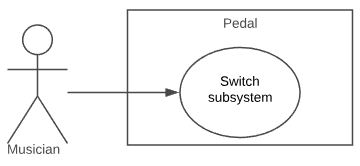
\includegraphics[width=.5\textwidth]{diagrams/use_cases/uc-switch.JPG}
                    \caption{Switch subsystem use case}
                    \label{fig:uc-switch}
                \end{figure}
        \clearpage
        \begin{table}[!ht]
            \centering
            \begin{tabular}{ l l  }
                Use Case & Switch subsystem  \\
                \hline \\
                Use Case Number & 1 \\ \\
                Summary & Musician can switch between the looping subsystem and the modulation subsystem. \\ \\
                Actor & Musician \\ \\
                Trigger & Hardware input: button or switch \\ \\
                
                Pre-Conditions & The pedal must be in either the looping subsystem or the modulation subsystem  \\ \\
                Post-Conditions & If the pedal was initially in the modulation system, it must be in the looping system. \\ 
                & If the pedal was initially in the looping system, it must be in the modulation system. \\ \\
                Assumptions & The pedal is powered on \\ \\
            \end{tabular}
            % \\
            % \caption{Use case: Switch subsystem}
            % \label{tab:uc-switch}
        \end{table}

        \paragraph{Start recording audio} 
        The user shall be able to record audio to playback later.
                    \begin{figure}[!ht]
                \centering
                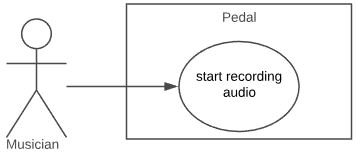
\includegraphics[width=.5\textwidth]{diagrams/use_cases/uc-record-start.JPG}
                \caption{Start recording audio use case}
                \label{fig:uc-record-start }
            \end{figure}
        \begin{table}[!ht]
            \centering
            \begin{tabular}{ l  l  }
                Use Case & Start recording audio  \\ \hline \\
                Use Case Number & 2 \\ \\
                Summary & Musician can start recording audio. \\ \\
                Actor & Musician \\ \\
                Trigger & Hardware input: pedal toggle \\ \\
                Pre-Conditions & The pedal must be in the looping subsystem. \\
                & The looping subsystem must not already be recording. \\ \\
                Post-Conditions & The looping subsystem will be recording incoming audio. \\ \\
                Assumptions & The user has audio input plugged in.\\
            \end{tabular}
            % \\
            % \caption{Use case: Start recording audio}
            % \label{tab:uc-record-start}
        \end{table}
        
        \clearpage
        \paragraph{Stop recording audio} 
            The user shall be able to record audio to playback later.
            \begin{figure}[!ht]
                \centering
                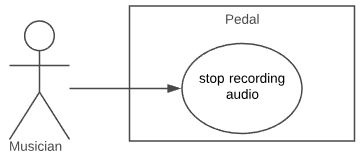
\includegraphics[width=.5\textwidth]{diagrams/use_cases/uc-record-stop.JPG}
                \caption{Stop recording audio use case}
                \label{fig:uc-record-stop }
            \end{figure}
            
            \begin{table}[!ht]
                \centering
                \begin{tabular}{ l  l }
                    Use Case & Stop recording audio  \\
                    \hline \\
                    Use Case Number & 3 \\ \\
                    Summary & Musician can stop recording audio. \\ \\
                    Actor & Musician \\ \\
                    Trigger & Hardware input: pedal toggle \\ \\
                    Pre-Conditions & The pedal must be in the looping subsystem. \\
                    & The looping subsystem must be recording audio. \\ \\
                    Post-Conditions & The looping subsystem will cache the recorded audio. \\ \\
                    Assumptions & The user has audio input plugged in.\\ 
                \end{tabular}
                % \\
                % \caption{Use case: Stop recording audio}
                % \label{tab:uc-record-stop}
            \end{table}
 
      
        \paragraph{Start audio playback} 
            The user shall be able to playback recorded audio.
            \begin{figure}[!ht]
                \centering
                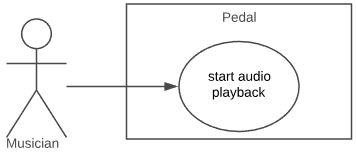
\includegraphics[width=.5\textwidth]{diagrams/use_cases/uc-play-start.JPG}
                \caption{Start audio playback use case}
                \label{fig:uc-play-start}
            \end{figure}
            \clearpage
            \begin{table}[!ht]
                \centering
                \begin{tabular}{l l}
                    Use Case & Start audio playback \\ 
                    \hline \\
                    Use Case Number & 4 \\ \\
                    Summary & Musician can start playing back audio. \\ \\
                    Actor & Musician \\ \\
                    Trigger & Hardware input: pedal toggle \\ \\
                    Pre-Conditions & The pedal must be in the looping subsystem. \\
                    & The looping subsystem must have audio cached. \\ \\
                    Post-Conditions & The looping subsystem will begin audio playback. \\ \\
                    Assumptions & None.\\ 
                \end{tabular}
                % \\
                % \caption{Use case: Start audio playback}
                % \label{tab:uc-play-start}
            \end{table}
            
            \paragraph{Stop audio playback} 
            The user shall be able to stop the playback recorded audio.
            \begin{figure}[!ht]
                \centering
                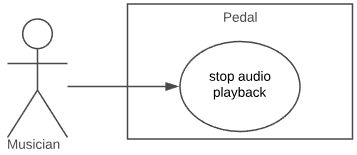
\includegraphics[width=.5\textwidth]{diagrams/use_cases/uc-play-stop.JPG}
                \caption{Stop audio playback use case}
                \label{fig:uc-play-stop}
            \end{figure}
            \begin{table}[!ht]
                \centering
                \begin{tabular}{l l}
                    Use Case & Stop audio playback \\ 
                    \hline \\ 
                    Use Case Number & 5 \\ \\
                    Summary & Musician can stop audio playback. \\ \\
                    Actor & Musician \\ \\
                    Trigger & Hardware input: pedal toggle \\ \\
                    Pre-Conditions & The pedal must be in the looping subsystem. \\
                    & The looping subsystem must have audio cached. \\
                    & The looping subsystem must be currently playing audio back \\ \\
                    Post-Conditions & The looping subsystem will stop audio playback. \\ \\
                    Assumptions & None.\\
                \end{tabular}
                % \\
                % \caption{Use case: Stop audio playback}
                % \label{tab:uc-play-stop}
            \end{table}
            
            \clearpage
            
            \paragraph{Select effect} 
            The user shall be able to select an effect.
            \begin{figure}[!ht]
                \centering
                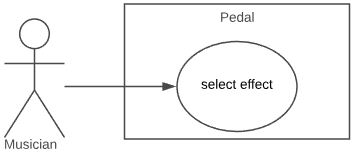
\includegraphics[width=.5\textwidth]{diagrams/use_cases/uc-select-effect.JPG}
                \caption{Select effect use case}
                \label{fig:uc-select-effect}
            \end{figure}
            
            \begin{table}[!ht]
                \centering
                \begin{tabular}{l l}
                    Use Case & Select effect \\
                    \hline \\
                    Use Case Number & 6 \\ \\
                    Summary & Musician can select an effect to use on the pedal. \\ \\
                    Actor & Musician \\ \\
                    Trigger & Hardware input: selector \\ \\
                    Pre-Conditions & The pedal must be in the modulation subsystem. \\
                    & The audio effect library must have effects. \\ \\
                    Post-Conditions & The modulation subsystem will load an effect to a cache. \\ \\
                    Assumptions & None.\\ \\
                \end{tabular}
                % \\
                % \caption{Use case: Select effect}
                % \label{tab:uc-select-effect}
            \end{table}            
            
            \paragraph{Start effect} 
            The user shall be able to start using an effect.
            \begin{figure}[!ht]
                \centering
                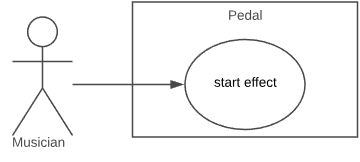
\includegraphics[width=.5\textwidth]{diagrams/use_cases/uc-effect-start.JPG}
                \caption{Start effect use case}
                \label{fig:uc-start-effect}
            \end{figure}
            \clearpage
            \begin{table}[!ht]
                \centering
                \begin{tabular}{l l}
                    Use Case & Start effect \\
                    \hline \\
                    Use Case Number & 7 \\ \\
                    Summary & Musician can start using an effect to modulate incoming audio. \\ \\
                    Actor & Musician \\ \\
                    Trigger & Hardware input: pedal toggle \\ \\
                    Pre-Conditions & The pedal must be in the modulation subsystem. \\
                    & The corresponding pedal toggle must have an effect cached. \\ \\
                    Post-Conditions & The modulation subsystem will start modulating incoming audio. \\ \\
                    Assumptions & An incoming audio signal exists.\\ \\
                \end{tabular}
                % \\
                % \caption{Use case: Start effect}
                % \label{tab:uc-start-effect}
            \end{table}     
            
            \paragraph{Stop effect} 
            The user shall be able to stop using an effect.
            \begin{figure}[!ht]
                \centering
                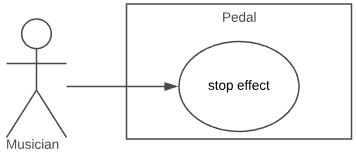
\includegraphics[width=.5\textwidth]{diagrams/use_cases/uc-effect-stop.JPG}
                \caption{Stop effect use case}
                \label{fig:uc-stop-effect}
            \end{figure}
            \begin{table}[!ht]
                \centering
                \begin{tabular}{l l}
                    Use Case & Stop effect \\
                    \hline \\
                    Use Case Number & 8 \\ \\
                    Summary & Musician can stop using an effect to modulate incoming audio. \\ \\
                    Actor & Musician \\ \\
                    Trigger & Hardware input: pedal toggle \\ \\
                    Pre-Conditions & The pedal must be in the modulation subsystem. \\
                    & An effect must be running. \\ \\
                    Post-Conditions & The modulation subsystem will stop modulating incoming audio. \\ \\
                    Assumptions & An incoming audio signal exists.\\ \\
                \end{tabular}
                % \\
                % \caption{Use case: Stop effect}
                % \label{tab:uc-stop-effect}
            \end{table}
            
\clearpage
\subsection{Composition viewpoint}

    \subsubsection{UML component diagram}
        \begin{figure}[!ht]
            \centering
            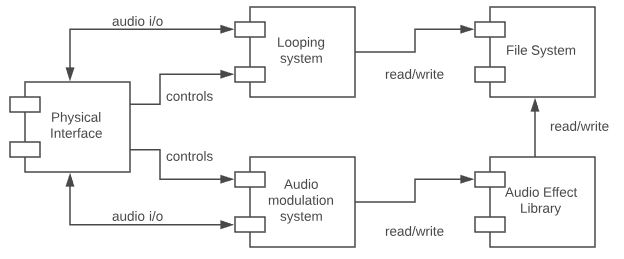
\includegraphics{diagrams/component-diagram.JPG}
            \caption{Component diagram}
            \label{fig:component}
        \end{figure}
    \subsubsection{Function attribute}
        The composition of the above entities creates the entire system to allow musicians to modulate incoming audio, or record and playback audio.
        
    \subsubsection{Subordinates attribute}
        The collection of the following entities work together to construct the working modulation/looping pedal: physical interface, looping system, audio modulation system, file system, and audio effect library.
\clearpage
\subsection{Dependency viewpoint}

    \subsubsection{UML dependency diagram}
        \begin{figure}[!ht]
            \centering
            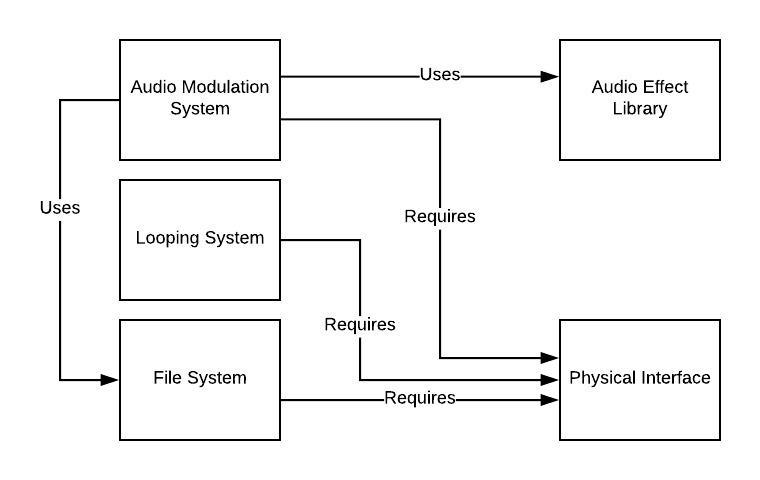
\includegraphics{diagrams/dependency-diagram.jpeg}
            \caption{Dependency diagram}
            \label{fig:dependency}
        \end{figure}
        
    \subsubsection{Dependencies attribute}
       Figure \ref{fig:dependency} shows the development dependencies for each subsystem. The first subsystems that can be designed are the Audio Modulation and Looping subsystems. The Looping subsystem design is independent from other components and can be developed at any time before the Physical Interface. The design of the Audio Modulation Subsystem is used to inform the Audio Effect Library and the File System designs. Once the software subsystems (Audio Modulation System, Looping System, and File System) are designed, work can begin on the Physical Interface design to create an interface that will adequately and efficiently control all three software subsystems.
        

\clearpage
\subsection{Interface viewpoint}
\begin{figure}[!ht]
    \centering
    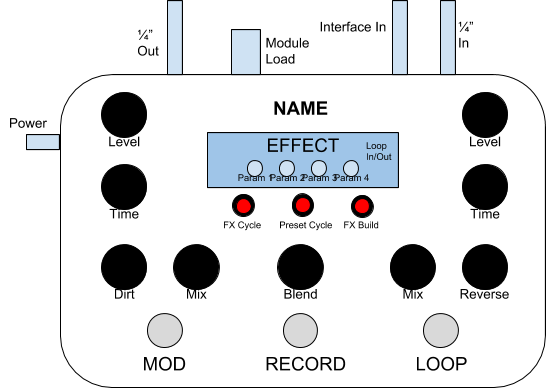
\includegraphics[width=.5\textwidth]{diagrams/pedal-diagram.png}
    \caption{Rough design diagram for the final product}
    \label{fig:pedal diagram}
\end{figure}

\subsection{Interaction viewpoint}

    \subsubsection{Looping System UML sequence diagram}
        \begin{figure}[!ht]
            \centering
            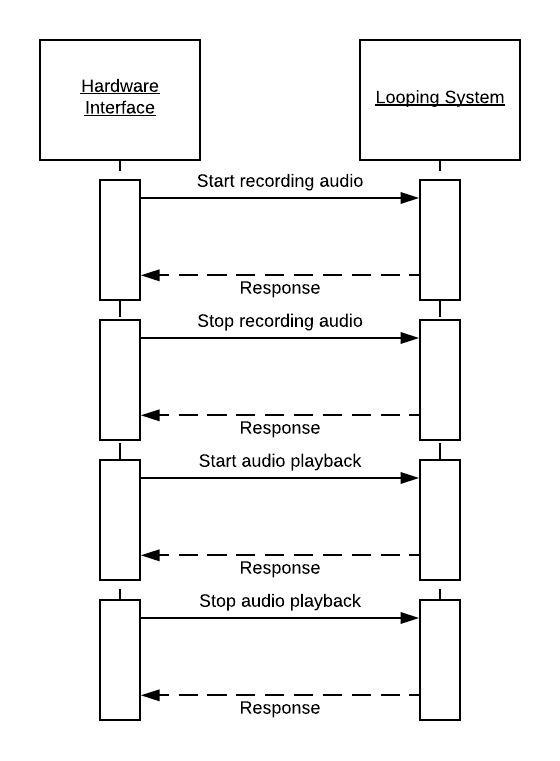
\includegraphics[width=.45\textwidth]{diagrams/looping-interaction.jpeg}
            \caption{Looping System sequence diagram}
            \label{fig:looping}
        \end{figure}
       Figure \ref{fig:looping} shows the intended interaction of the Hardware Interface and Looping Subsystem. Physical controls on the Hardware Interface correspond directly to the functionality of the Looping system. Creating a one to one relationship between the physical controls on the hardware and the software functionality they control should facilitate intuitive control while affecting the Looping System.

    \subsubsection{Audio Modulation System UML sequence diagram}
        \begin{figure}[!ht]
            \centering
            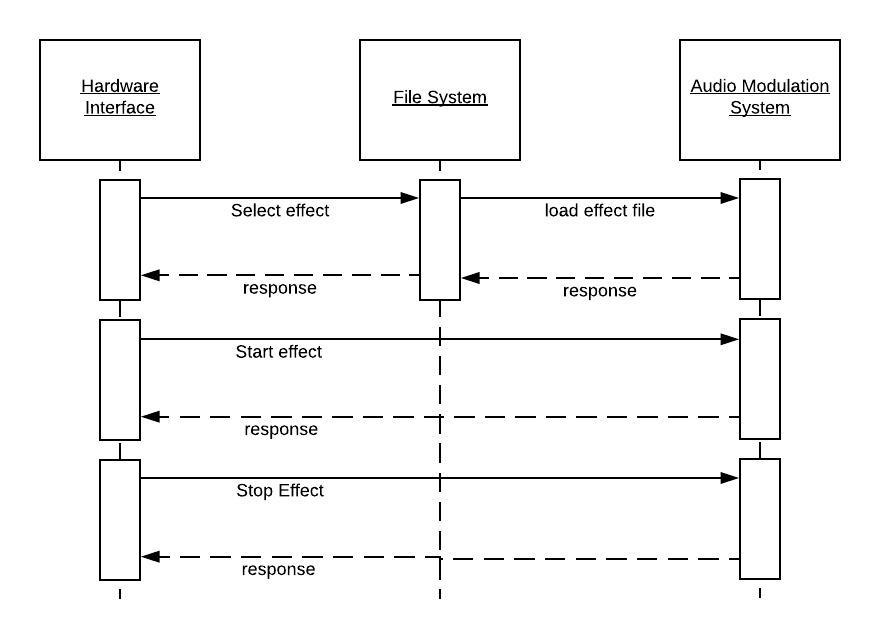
\includegraphics[width=.75\textwidth]{diagrams/modulation-interaction.jpeg}
            \caption{Audio Modulation System sequence diagram}
            \label{fig:modulation}
        \end{figure}
        Figure \ref{fig:modulation} illustrates the intended interaction between the Hardware Interface and the Audio Modulation System.
        

%\subsection{Algorithm viewpoint}
%Many of the algorithms that will need to be used already exist in the libraries we will be using. For example, csound has a built in low pass filter. 

\subsection{Resource viewpoint}
    The resources that may be present in the product, but are not part of the design are:
    \begin{itemize}
        \item External display device.
        \item Open source libraries.
        \item Any behavior related to stretch goals.
    \end{itemize}
\newpage
\bibliographystyle{IEEEtran}
\bibliography{./refs.bib}


\end{document}
